\chapter{Evaluation} % English: Evaluation
\label{chap:evaluation}

This chapter summarizes the results of the experiments. At the center of the
evaluation stands the comparison of the energy consumption of the default
\emph{Contiki}-\ac{RPL} and version with added persistance of routing
information. Another important point is how the network topology behaves in the
different configuration and how the network reacts to resetting nodes. For this,
the power consumption of the individual nodes and the complete network, the stability
of the \ac{DAG} and the performance of the network are evaluated.

\section{Firmware Configurations}
\label{sec:confs}

For the firmware, three different modes have been evaluated. The first mode uses
the default \emph{Contiki}-\ac{RPL} (N), the second uses the hardened implementation with
only the storing of persistent state enabled (H) and in the third mode additionally
the sanity of the routing information is checked using \acp{UID} and the clock
values of the neighboring nodes (HS). Each mode is tested for a network where a
reset occurs (R) and for a network where no resets occur. From this result 6
different variants of the experiment which are shown in \autoref{tab:variants}.

\begin{table}[h]
  \centering
  \caption{Experiment configurations}
  \begin{tabular}{r c c c}
    \toprule
    Test run & Hardened & Sanity & Resets \\
    \midrule
    N   &   &   &   \\
    R   &   &   & X \\
    H   & X &   &   \\
    HR  & X &   & X \\
    HS  & X & X &   \\
    HSR & X & X & X \\
    \end{tabular}
  \label{tab:variants}
\end{table}

\section{Influence of Environmental Factors}

When evaluating the data obtained from \fitlab some environmental factors that
have an influence on wireless transmissions have to be taken into account.

\subsection{Radio Interference}

The radio of the \emph{M3} node uses the 2.4 GHz \ac{ISM} bands. One problem
with this is, that this shared spectrum suffers from interference with other
users since it is widely used for other network applications (e.g. \emph{WiFi}).
This means that interference with surrounding devices in the building and with
other experiments in the testbed is legitimate concern. As long as other devices
use some form of \ac{MAC} that is compatible with the one used in IEEE 802.15.4,
this is less of a problem since different senders is able to
coordinate their transmissions to some degree. Because the complete networking
stack the \ac{ON} uses can be user-defined, as is the case with all software
running on the \ac{ON}, this may not always be given.

In the case of previous experiments by Müller et al. \cite{mueller2017}, this
problem was responded to by only running the experiments at night time, where
other senders are less active. In the case of \fitlab, where experiments
may run unsupervised, this is likely not a valid strategy. Another mitigation that
has been performed is to select channel 16 in the 2.4 GHz spectrum in use for
IEEE 802.15.4 and then capturing traffic that can be seen on this channel. Also,
the \ac{API} allows to monitor if other experiments are scheduled during an
experiment and a more appropriate time can be selected instead.

Since we use almost all nodes that are available for experiments and not down
for maintenance, other experiments are effectively prevented from interfering
with ours. Selecting channel 16, in this case, has also proven to be effective in limiting
interference from other networks.

\subsection{Signal Propagation}

As can be seen in \autoref{fig:testbed}, the test network is located on the floor
of a building. This building has multiple floors. The larger part of the
building on the right is separated from the smaller part of the building on the
left in some places by a wall. There are a few pillars between some of the test
nodes. All of them present obstacles for the propagation of the signal. As for the influence
they have on the experiment, it can be noted that the positions of all obstacles
remains constant during and between each experiment. However, the physical topology
(e.g. which nodes are neighboring each other) changes compared to a strictly
linear topology as suggested by the map.

\section{Topology of the RPL Network}

The topology of the network does have a large influence on how much the network
is affected by a resetting node, as was previously shown by Kulau et al. \cite{kulau2017energy}.
For the different runs of the experiment to remain comparable, it is necessary
that under the same conditions the network obtains a similar topology.

\subsection{Ideal Network Topologies}

As previously established, the affect resetting nodes have on the network
depends on the position and role of the node inside the network.

In a tree-like topology as depicted in \autoref{fig:treetop}, nodes have at most
one alternative parent and the entire sub-tree underneath the resetting node
will be affected as they lose their default route to the root node.

For a mesh-like topology, such as in \autoref{fig:meshstar}, the network may be
able to quickly recover after the nodes have selected one of their alternative
parents.

While these topologies serve the purpose of illustrating which factors play into
the behavior of a recovering network, it is not easily possible to recreate such
topologies in a real-wold scenario, since the topology of the network is limited
by the different configurations \fitlab offers.

\begin{figure}
  \centering
  \begin{tikzpicture}[<-,>=stealth', level/.style={sibling distance = 5cm/#1, level distance = 1.5cm}, font = \small, every node/.style={circle,draw}]
    \node {1}
    child { node {2}
      child { node {5}
        child { node {11} }
        child { node {12} }
      }
      child { node {6}
        child { node {12} }
        child { node {13} }
      }
    }
    child { node {3}
      child { node {7}
      }
      child { node {8}
        child { node {14} }
        child { node {15} }
      }
      child { node {9}
      }
    }
    child { node {4}
      child { node {10}
        child { node {16} }
        child { node {17} }
        child { node {18} }
      }
      child { node {11}
        child { node {19} }
      }
    };
  \end{tikzpicture}
  \caption{Tree topology}
  \label{fig:treetop}
\end{figure}

% TODO build in \latex \tikz
\begin{figure}
  \centering
  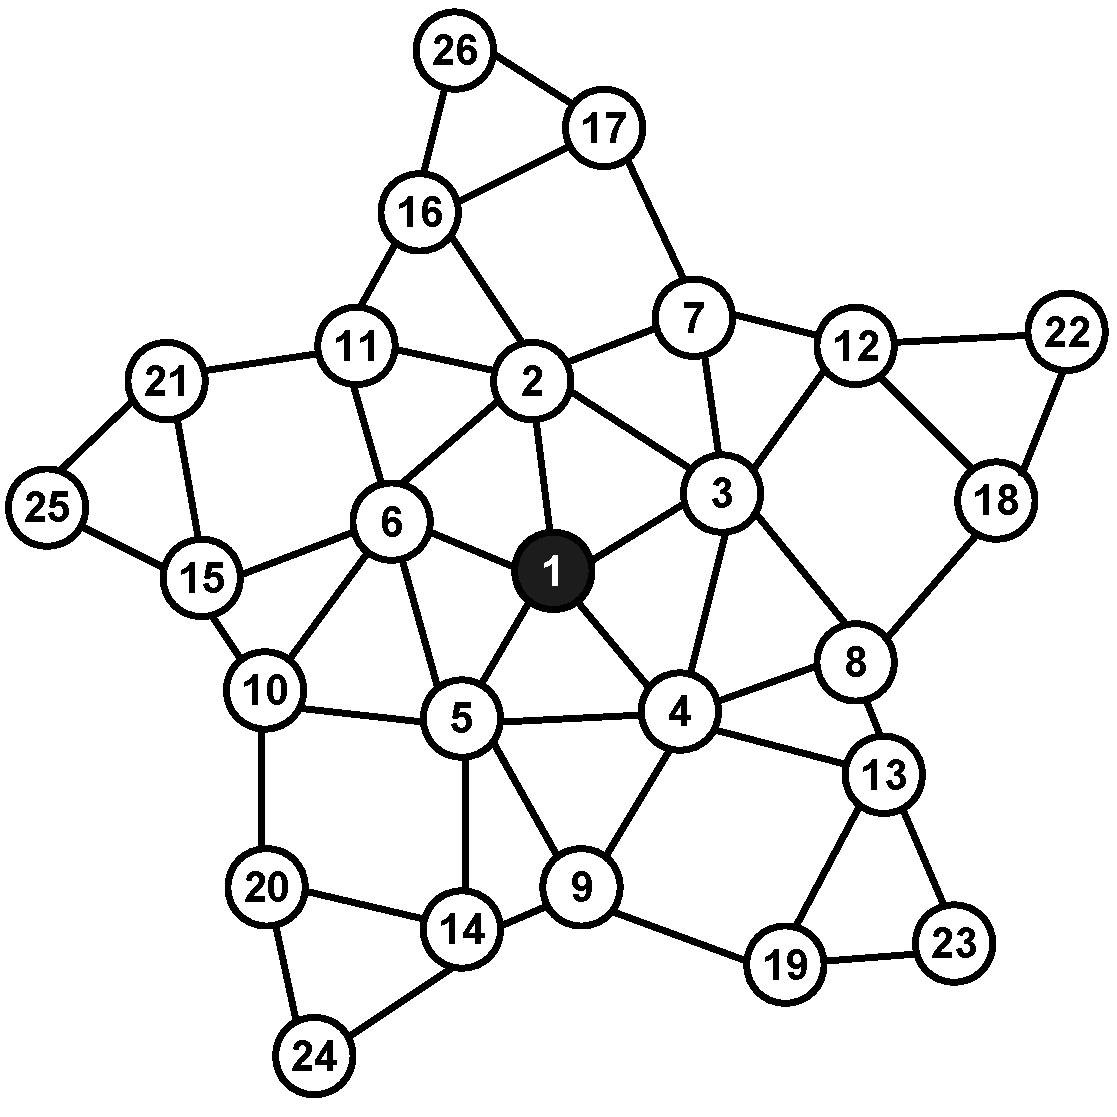
\includegraphics[width=.5\textwidth]{../images/sim_star_new.pdf}
  \caption{Star mesh topology \cite{mueller2017}}
  \label{fig:meshstar}
\end{figure}

\subsection{Measured Topology}

Each topology resulting from any experiments in \fitlab converges upon a very similar
\acs{DAG}. An example of such a \ac{DAG} is shown in \autoref{fig:dagexample}.
One thing that can be observed is that the resulting tree has up to 6 layers.
It should be noted that most nodes are an equal distance to another as displayed
in \autoref{fig:testbed} and the links can be assumed to be of similar quality.

\begin{figure}
  \centering
  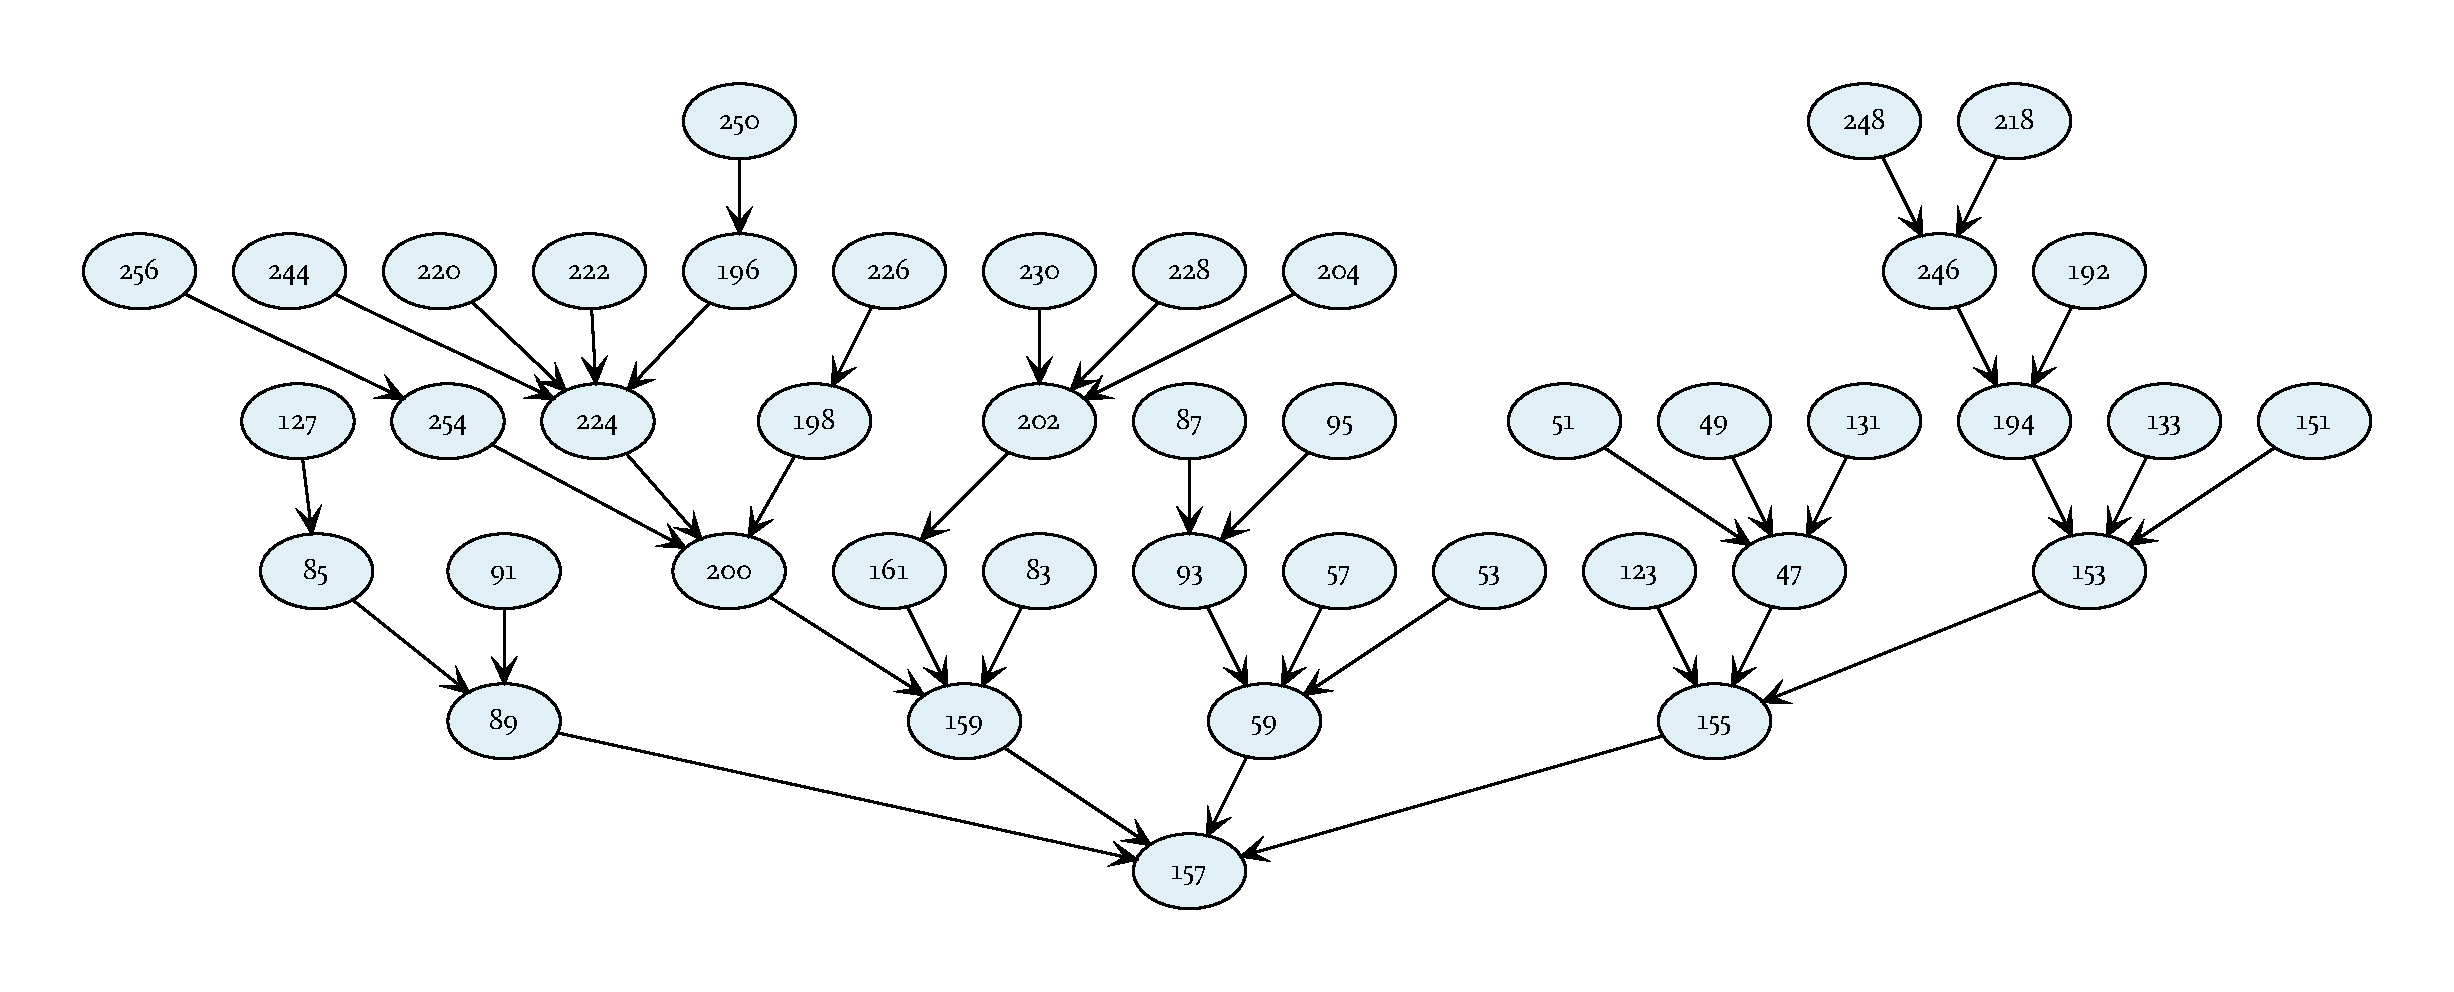
\includegraphics[width=\textwidth]{../images/dag.pdf}
  \caption{An example of a DAG generated for the configuration used in the evaluation}
  \label{fig:dagexample}
\end{figure}

\subsubsection{Relationship to the Physical Topology}

One common property of the \ac{DAG}s is that node 159 is the root of the largest
sub-tree. When comparing the nodes of this sub-tree to their positions on the
map, one noticeable property of this sub-tree is that it even contains nodes that
have a closer physical distance to nodes from other sub-trees. In the depicted
tree an example would be node 196 joining the sub-tree of 159 instead of a
acquiring the directly neighboring node 155 as a parent. When comparing to the
shape of the surrounding building these two nodes are divided by two outside
facing walls of the surrounding building, while the path across 159, 200 and 224
is only obstructed by a dry-wall which presents less of an obstacle to the radio
signal.

\subsubsection{Selecting a Node to Reset}

Initial evaluations of the resulting topologies give an indication to which node
needs to reset to have a measureable effect on the network. Node 200 has been
selected to be reset during a single random time during the phases with resets,
R, HR and HSR. The reasons for this are that node 200 has a large enough sub-tree in
most runs of the experiment to affect enough nodes and because it is the node
that is most frequently selected as a preferred parent when connecting the two
halves of the building.

\subsection{Route Stability}

The stability of the network is determined by how stable the conditions are on
which the routing protocol bases its decisions. For a network where resets
occur, these conditions will change upon the reset of a node and the routing
protocol reacts to this situation. Therefore, the number of changes of the
routing decisions is a measure of the stability of the network created by the
routing protocol.

\begin{figure}
  \centering
  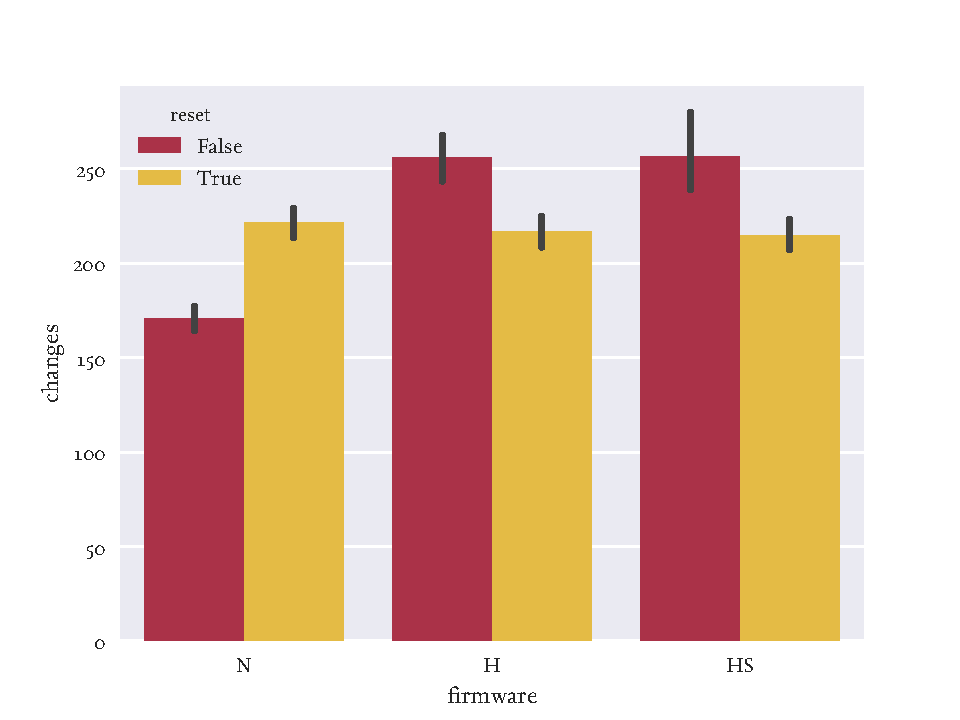
\includegraphics[height=.3\textheight]{../images/stability.pdf}
  \caption{Number of changes of the default route of any node during a phase}
  \label{fig:stability}
\end{figure}

\autoref{fig:stability} shows the number of changes of the default route of any
node during each phase of an experiment. The default implementation in phase N
causes the fewest changes if no single node resets occur. The hardened
implementations of H and HS on the other hand lead to more changes. This may be
due to the processing, or restoring and invalidating a previous invalid state from
persistent memory.

The number of changes for the hardened implementations during a phase with
single node resets is smaller than for the default implementation. This means
that the hardened implementations recover more easily from single node resets
than the default implementation does.

\subsubsection{Relation to Location}

\autoref{fig:hmroutes} shows a heat-map of the distribution of default routes
during each phase. Each cell results from the number of times the route has been
selected at the end of an interval of 10 seconds during the phase of an
experiment. This number was then then normalized by the length of the phase
during the experiment, since the length of a phase may vary due to variations in
how fast the test-lab reacts to instructions given by the orchestration
component. Thus, routes that are more often selected are shown in a darker hue,
while routes that are rarely selected are shown in a lighter hue. 

\begin{figure}
  \centering
  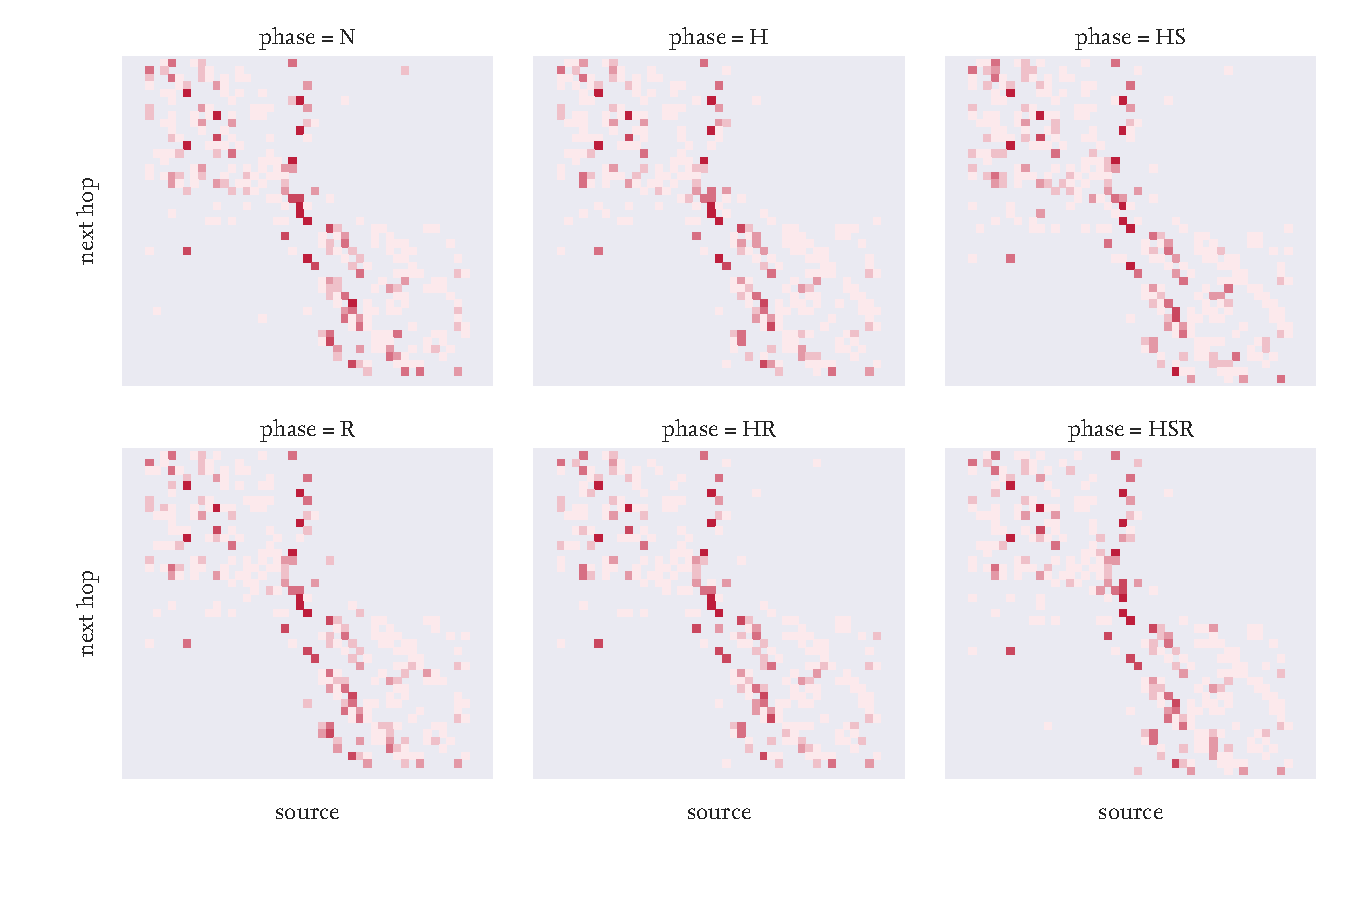
\includegraphics[width=\textwidth]{../images/routes.pdf}
  \caption{Heat-map of the normalized choice of default routes for the different
    phases}
  \label{fig:hmroutes}
\end{figure}

The most noticeable thing about the these maps is that the distribution of
routes of routes between the different phases does not vary much, in that the
maps are almost identical. One thing to conclude from this is that the choice
of the \ac{DAG} is not altered in a relevant way by adding the persistance mode
in phase H or additionally validating \acp{UID} in phase HS. This means that
that there is not enabling the hardened implementation in regard to the choice of
an optimal \ac{DAG}.

Another thing to be noted is that the when viewing each row of the map, some
nodes show a distribution of routes which is very dense for a small number of
different neighbors while others do not have such routes. When compared to the
topology of the \ac{DAG}, the nodes that offer more stable routes are generally
inside nodes of the tree (e.g. not leaves). Nodes that tend to change
routes more join the tree as nodes.

The comparison of the phases have resets with their counterparts yields that there
are more changes between the N and the R phase than are between the H and the HR
and the HS and the HSR phases. From this it can be interpreted that more route
changes may have occurred during the reset of the node in phase R. This would
mean that the network is in a more unstable state during R than in HR and HSR.

%\subsubsection{Relation to Rank and Number of Neighbors}
%
%\autoref{fig:rankvsneighvschanges} shows the pairwise relationship of the rank
%of a node, its number of neighbors and the number of changes of its preferred
%parent selection.
%
%% TODO create new figure
%
%%\begin{figure}
%%  \centering
%%  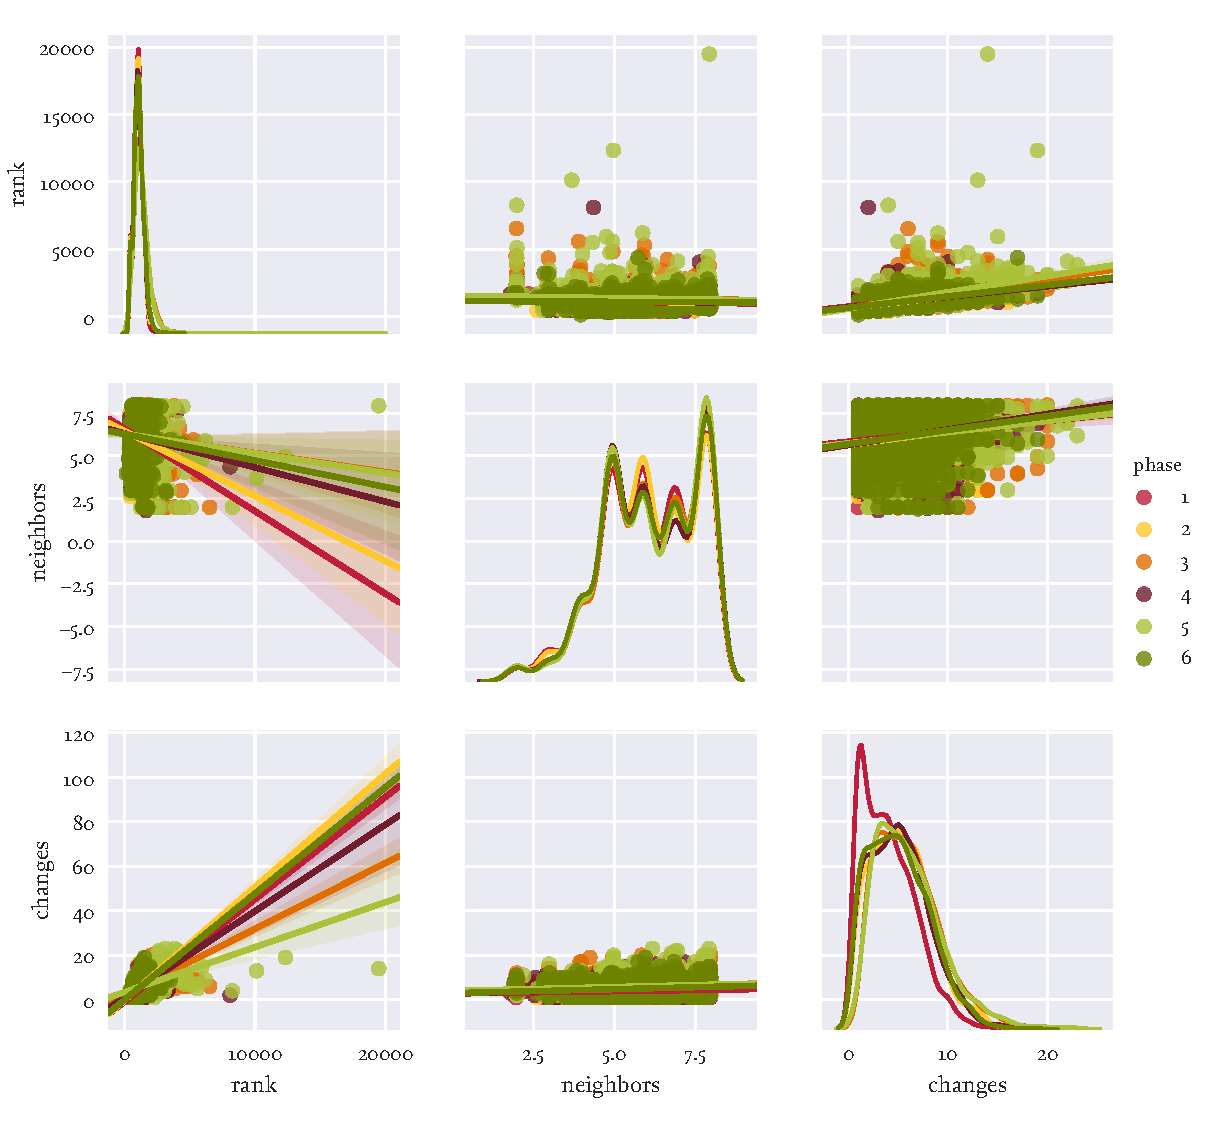
\includegraphics[width=\textwidth]{../images/changes.pdf}
%%  \caption{Rank, default parent changes, number of neighbors}
%%  \label{fig:rankvsneighvschanges}
%%\end{figure}
%
%With increased rank, the number of changes of the preferred parent increases.
%This may cause an increase in energy consumption. One possible explanation may
%be that the possible number of nodes that may fail along the path to the sink is
%increased when a node has a higher rank. This is supported by the fact that the
%increase in changes is higher for the phases that include resetting a node. As
%such it can be expected to see a noticeable increase in power consumption for
%these phases (see \autoref{fig:consum-rank.pdf}).

\subsection{Convergence Time}

When considering the resulting routing topology, the time it takes the network
to converge upon one topology is also of interest. A larger amount of
routing messages will have to be transmitted, the longer some single node in the
network takes to acquire a preferred parent.

\autoref{fig:convtime} shows the convergence time of the network for each phase.
The phases without resets are grouped to the left and on the right are displayed
the phases with resets.

\begin{figure}
  \centering
  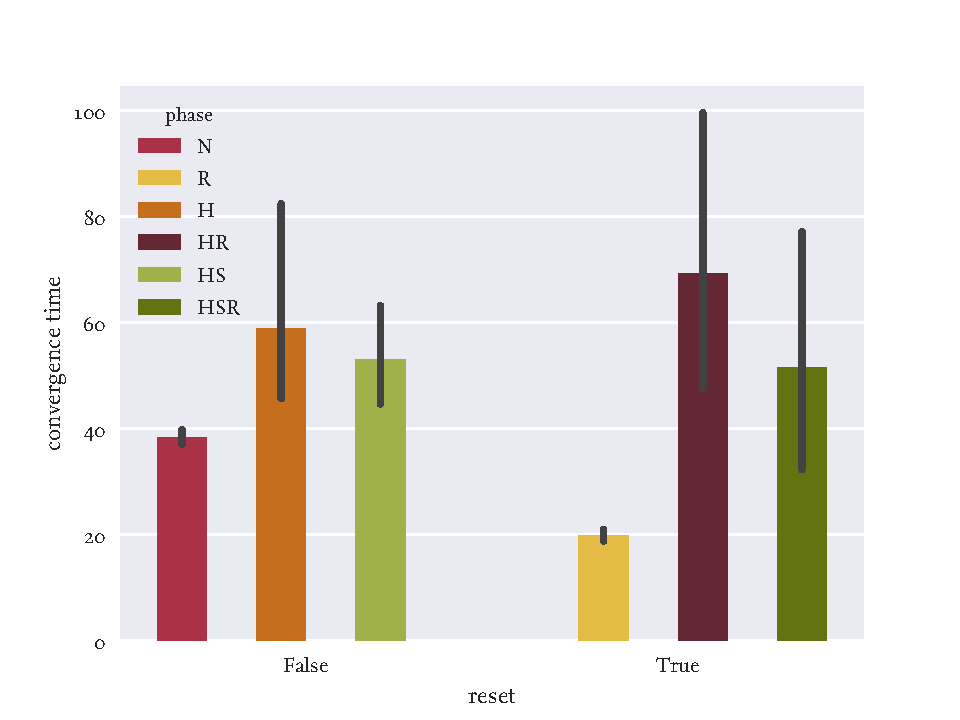
\includegraphics[height=0.3\textheight]{../images/convergence.pdf}
  \caption{Network convergence time for each phase}
  \label{fig:convtime}
\end{figure}

It is noticeable that both the H and HS phases, which use the hardened
implementation, have generally longer convergence times than the default
implementation of \ac{RPL}. In the case of the restoration of the routing state
from persistent memory, as in phase R and HS, all previously recorded \ac{DIO}
messages will be replayed to the \ac{RPL} module of \emph{Contiki}. This implies
that the time it takes to process these messages and make changes to the saved
\ac{DAG} and routing table adds to the time it takes to choose a preferred
parent and therefore lengthens the network formation time. It can be assumed
that much of this time is spend writing and reading this data from the peristant
memory.

In the case of the HS and HSR phases, additional \ac{DIO} messages are
exchanged to verify the stored routing information and messages before restoring
them. These messages contain \acp{UID} to identify the information and measure
the freshness of the information using the clock the implementation keeps for
the local routing information. Presumably, the time it takes to exchange these
messages further adds to the delay until a suitable preferred parent is selected
for each node.

Another thing that is remarkable is how much the convergence time varies for the
H and HS phases compared to the phases without the hardened implementation,
regardless of whether there are resets or not. As a consequence, the network
forms in a more reliable manner in the default implementation.

An interesting observation about the difference in the convergence time between the
phases with resets and those without is that generally the convergence time is
shorter for a network with resets. It would be expected that the inverse of this relation would
be the case. The exact reason for this can only be speculated upon. If a reset
occurs during the initial formation of the \ac{DAG} during a phase, the
resetting node might not partake in the formation of the network. This then
would mean that less alternative paths inside the network exist from which to
choose which might lead to the network converging faster.

% TODO network convergence time derectly after reset


\section{Energy Consumption}

% TODO error from measuring 2nd phases --> indirect comparison by # messages ...
This section discusses the energy consumption of the test
network and how it changes based on the implementation in use and whether a single
node reset occurs. \autoref{fig:consphases} shows the total energy consumption
of the network during the different phases. Nodes 200 and 157 have been excluded
since they act as the resetting node and the root node.

\begin{figure}
  \centering
  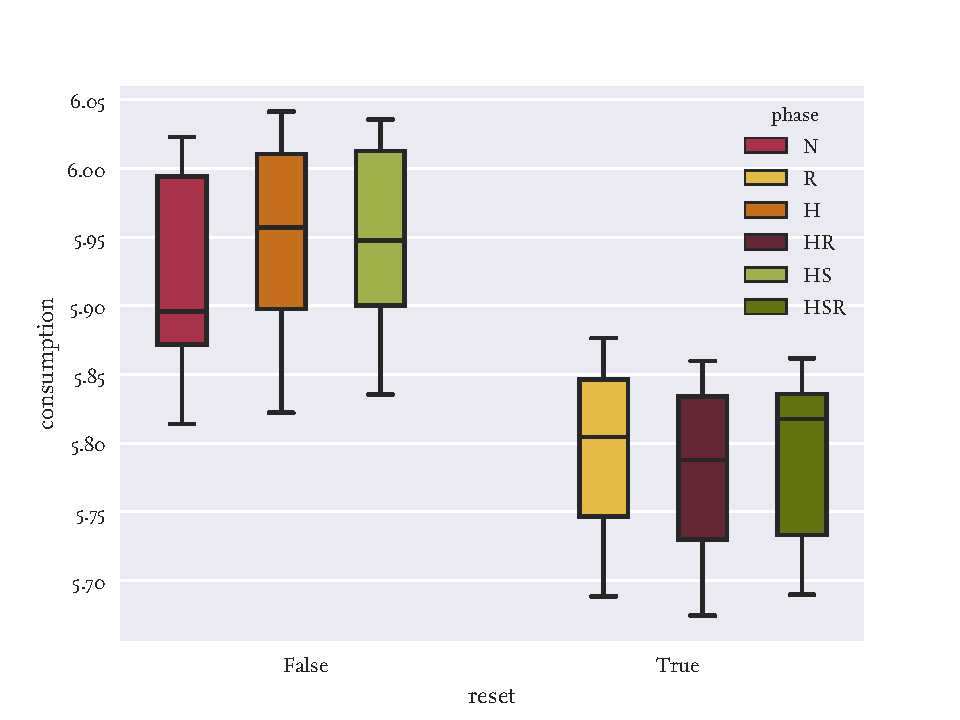
\includegraphics[height=0.3\textheight]{../images/consumption-phases.pdf}
  \caption{Total consumption except nodes 200 and 157}
  \label{fig:consphases}
\end{figure}

For a network in which no resets occur, the consumption of the default
implementation (N) is significantly lower than for both versions of the hardened
implementation (H, HS). One possible factor in this may be the energy spend on writing
the persistent state to the flash memory. Another may be the additional
computing time spend on processing the restored state and in case of the HS
phase, the exchange of \ac{DIO} messages.

This effect is amortized when recovering from a reset in the phases HR and HSR,
where the default implementation uses more energy than the hardened version (HR).
For instances, the extended hardened implementation (HSR) uses less power than
the default implementation, but the mean of the consumption is higher for HSR.
This means that the additional exchange of messages to verify the state stored
in persistent memory consumes more energy on average than the restoring of the
persistent state saves.

\subsubsection{Constant error between consecutive phases}

The comparison of the phases in which no resets occur (N, H, HS) versus the
phases with resets (R, HR, HSR) yields, that a smaller energy consumption is
measured for the phases with resets. 

For each firmware, the phase with and without resets run consecutively. For each
series of measurements for each individual node the power consumption of each
second phase is smaller over the complete duration of the phase. This leads to
the conclusion that this behavior is not triggered by the single node reset,
but rather caused by an external factor.

For this reason, the measured values of the energy consumption of the
individual phases are only valid for comparison between phases that either have
resets or do not. For the comparison of the phases that use the same firmware
(e.g. N and R) other variables can be used, such as the number of protocol
messages and the number of changes of the preferred parent.

%TODO measurement sequence

\subsection{Consumption of the DAG Root and Resetting Node}

\autoref{fig:cmpsinkreset} shows the total consumption of the network, except for
the sink node and the resetting node. Node 123 is shown for comparison as it is
close to the average of the consumption of all other nodes.

\begin{figure}
  \centering
  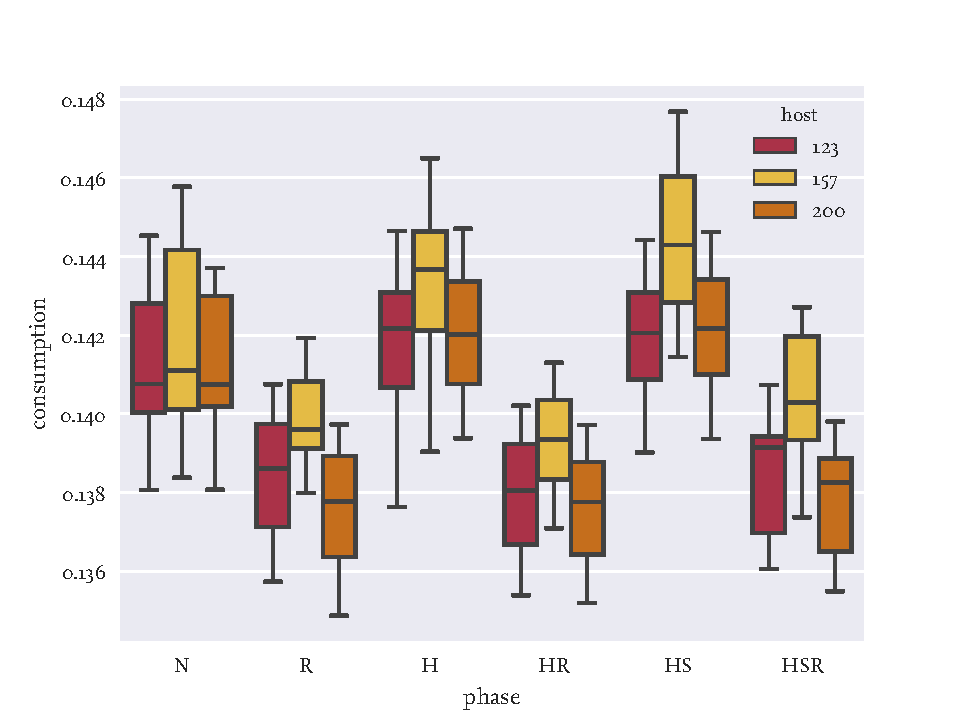
\includegraphics[height=0.3\textheight]{../images/consumption-hosts.pdf}
  \caption{Energy consumption for the sink node and the resetting node}
  \label{fig:cmpsinkreset}
\end{figure}

When viewed separatly, the energy consumption of these nodes varies widely from
the other nodes and from each other as seen in \autoref{fig:cmpsinkreset}. In
the case of the sink node, this is because, to minimize packet loss, its radio
is forced to the \ac{RX} state and it acts as the \ac{UDP}-sink and thus has to
process many packets. The resetting node can be expected to consume much less
power while it is resetting, since a restart involves power-cycling the node.
Thus, for the phases with resets (R, HR, HSR), the consumption is lower for node
200 and 157 consumes significantly more energy than the average node. Such a
node would typically be powered from the power grid.

%\subsection{Relation to Rank}
%
%% TODO
%
%As can be viewed from \autoref{fig:relconsum}, the energy consumption increases
%with the rank for HS and HSR. For the N and H, this relationship is inverted.
%
%\begin{figure}
%  \centering
%  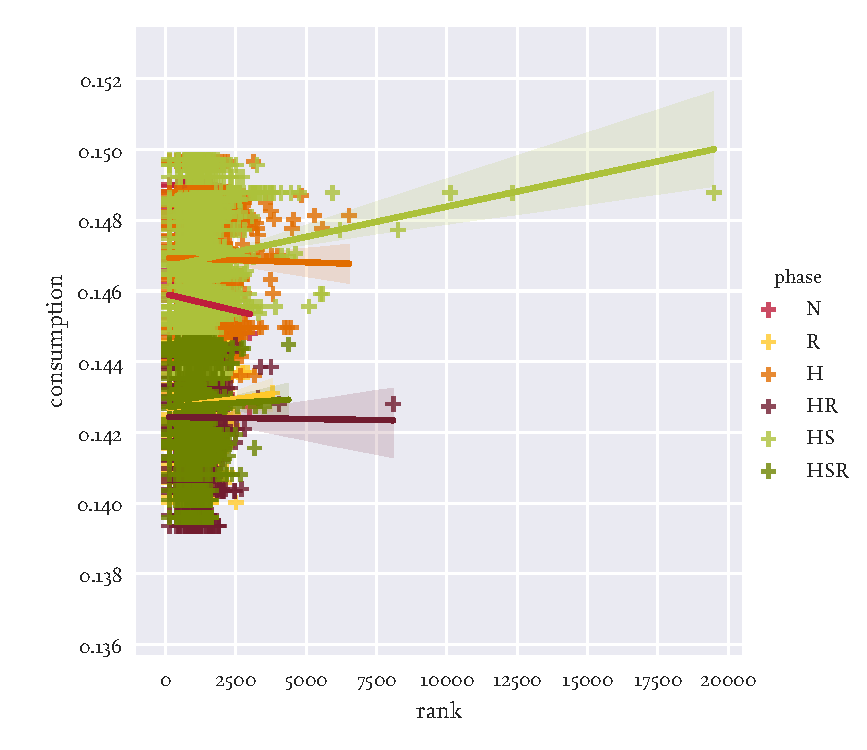
\includegraphics[height=0.4\textheight]{../images/consumption-regress.pdf}
%  \caption{Relation of rank and consumption of a node}
%  \label{fig:relconsum}
%\end{figure}

\subsection{Relation to Position inside the Testbed}

\autoref{fig:posenergy} displays the positions of the nodes inside the testbed.
Every cell shows a color representing the relative energy consumption associated with
that node. Lighter colors represent a lower energy consumption, whereas darker
colors represent a higher energy consumption.

\begin{figure}
  \centering
  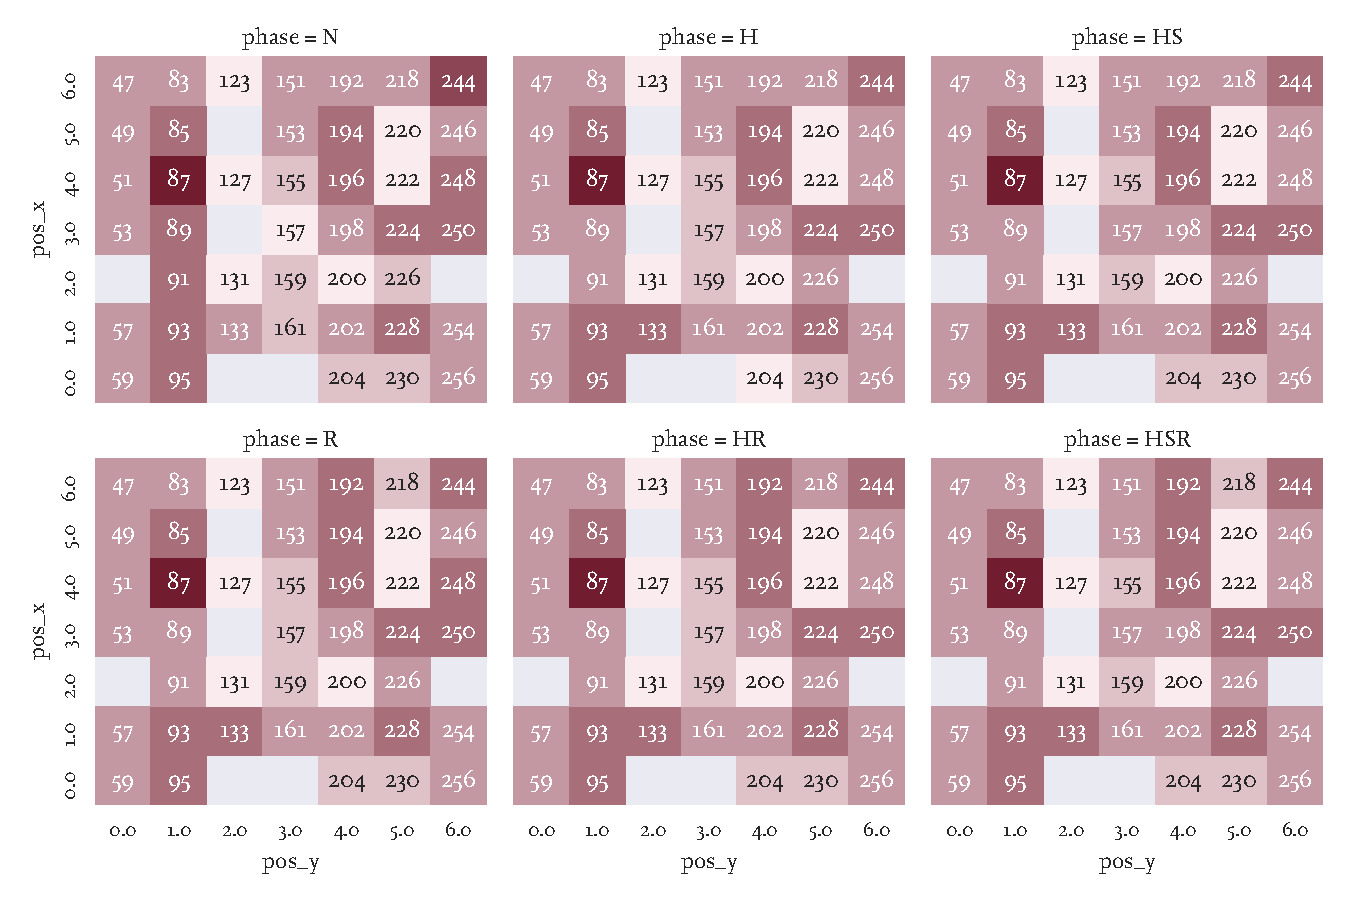
\includegraphics[width=0.4\textheight]{../images/consumption-nodes.pdf}
  \caption{Energy consumption of nodes arranged by their position}
  \label{fig:posenergy}
\end{figure}

One noticeable thing about this distribution is that node 87 has the highest
energy consumption in all phases. When looking at the \ac{DAG}, this node is
mostly located at a lower rank. Nodes that are physically located closer to the
root node 157, tend to have a lower energy consumption than surrounding nodes.
A wall separates the nodes 192, 194 and 196 from 157. This coincides with these
nodes having a higher energy consumption.

\section{Network Performance}

In this section, the network performance and the control overhead for the
different phases is evaluated.

\subsection{End-to-End}

\autoref{fig:perf} shows the average end-to-end delay for all nodes during each
phase of the experiment. While in phase H, shorter delays are possible. At the
same time, the distribution varies more. With the added sanity checks in phase
HS, the distribution is more focused around 2 ms. The default implementation in
N lies somewhere in-between the two.

%\begin{figure}
%  \centering
%  \subfloat[delay]{{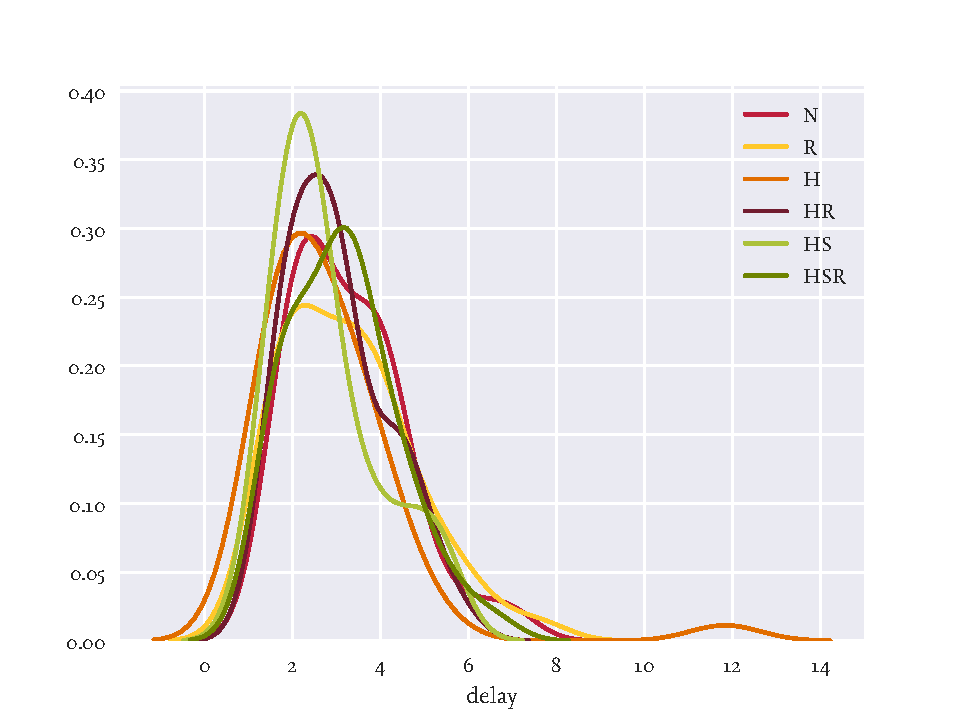
\includegraphics[width=.5\textwidth]{../images/performance-delay.pdf}}}%
%  \qquad
%  \subfloat[jitter]{{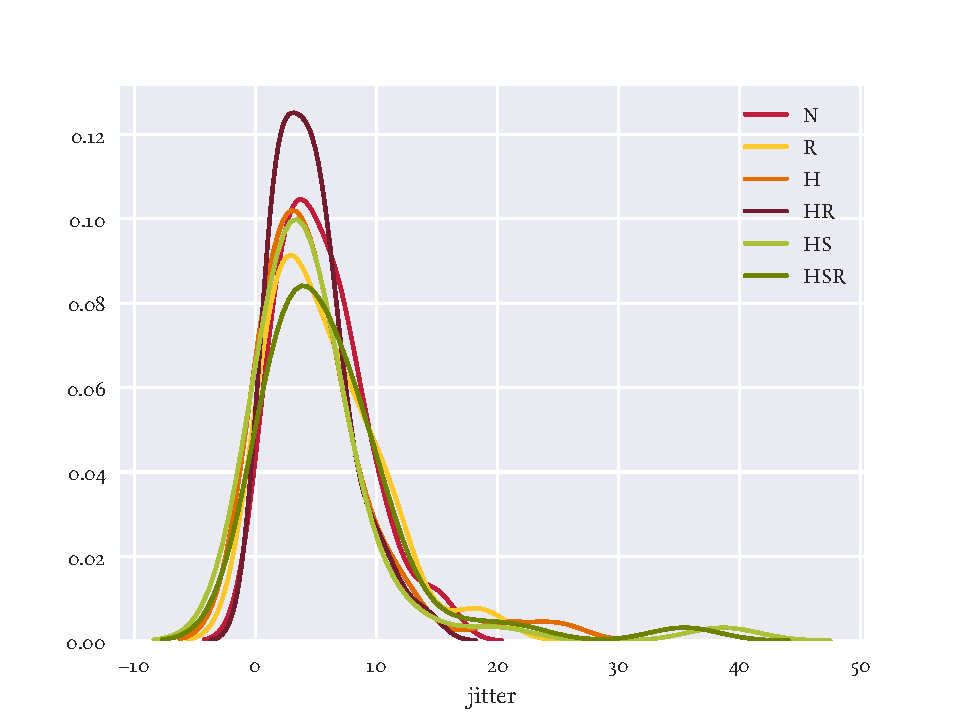
\includegraphics[width=0.5\textwidth]{../images/performance-jitter.pdf}}}%
%  \subfloat[loss]{{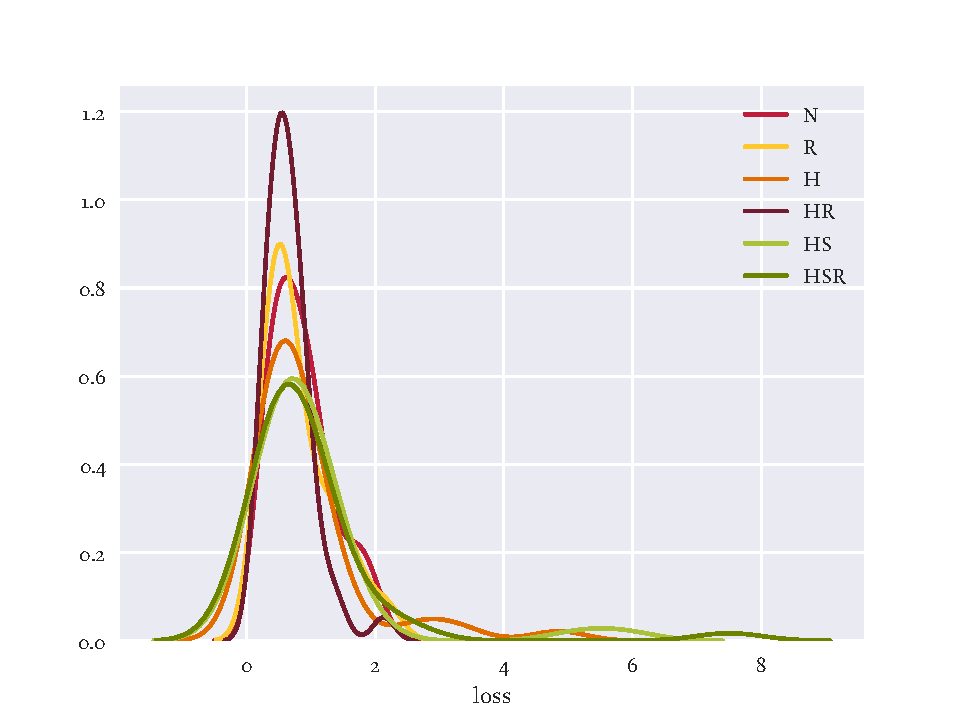
\includegraphics[width=0.5\textwidth]{../images/performance-loss.pdf}}}%
%  \caption{Delay, jitter, loss for each phase}
%  \label{fig:perf}
%\end{figure}
\begin{figure}
  \centering
  \subfloat[delay]{{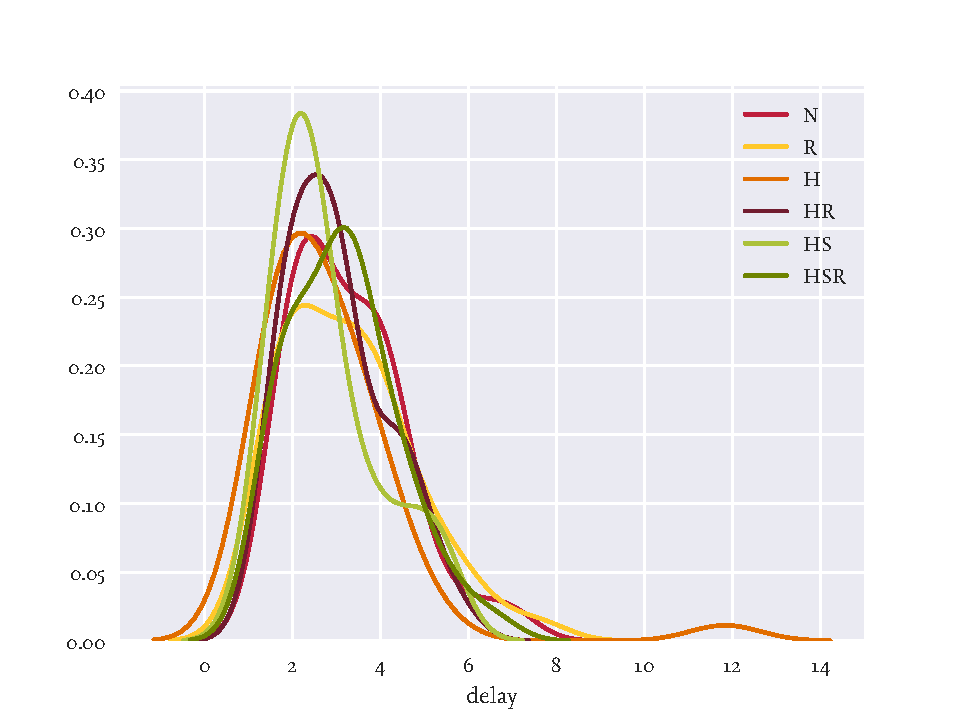
\includegraphics[width=.5\textwidth]{../images/performance-delay.pdf}}}%
  \subfloat[loss]{{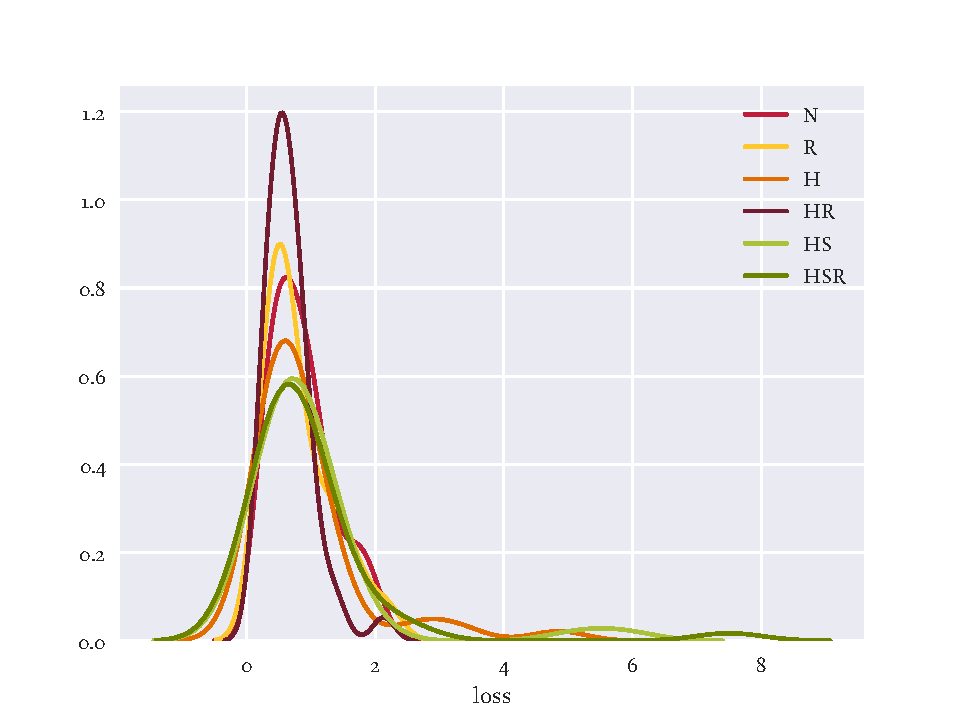
\includegraphics[width=.5\textwidth]{../images/performance-loss.pdf}}}%
  \caption{End-to-end delay and package reception rate}
  \label{fig:perf}
\end{figure}

The packet loss during each phase is displayed in \autoref{fig:perf}. For a
scenario without single node resets, the default implementation fares best,
while in a scenario with single node resets the hardened version without the use
of \acp{UID} looses the fewest packets. If additionally the sanity checking
of the persistent state is enabled, the most packets are lost.

One possible explanation for this is that if the persistent state is directly
restored, most of the time this state is sufficient for the forwarding of newly
arriving packets. If the node must first validate the saved state, it looses
time during which arriving packets may be dropped. This would suggest that the
validation of the saved state is actually slower than the default method of
recovery.

\subsection{Control Overhead}

The number of messages that need to be emitted during the repair operations of
the \ac{DAG} determines the utilisation of the radio of the node. It is to be
expected that a large part of the energy consumption of the each node is
determined by the number of messages it emits. Thus, when evaluating the
efficiency of the different implementations and the impact of the single node
resets, the overhead of messages that are transmitted by the implementation
serves an important measure.

\autoref{fig:overhead} shows the overhead created by control messages that were created
during each phase by message type. For each type, the default implementation
creates the fewest additional messages of any type, while the number of messages
is the highest for the implementation used in HS. This may be attributable to
the higher number of messages exchanged during the validation process. The
larger number of overhead created during phase H is likely due to an old state
being restored from previous runs and then invalidated.

\begin{figure}
  \centering
  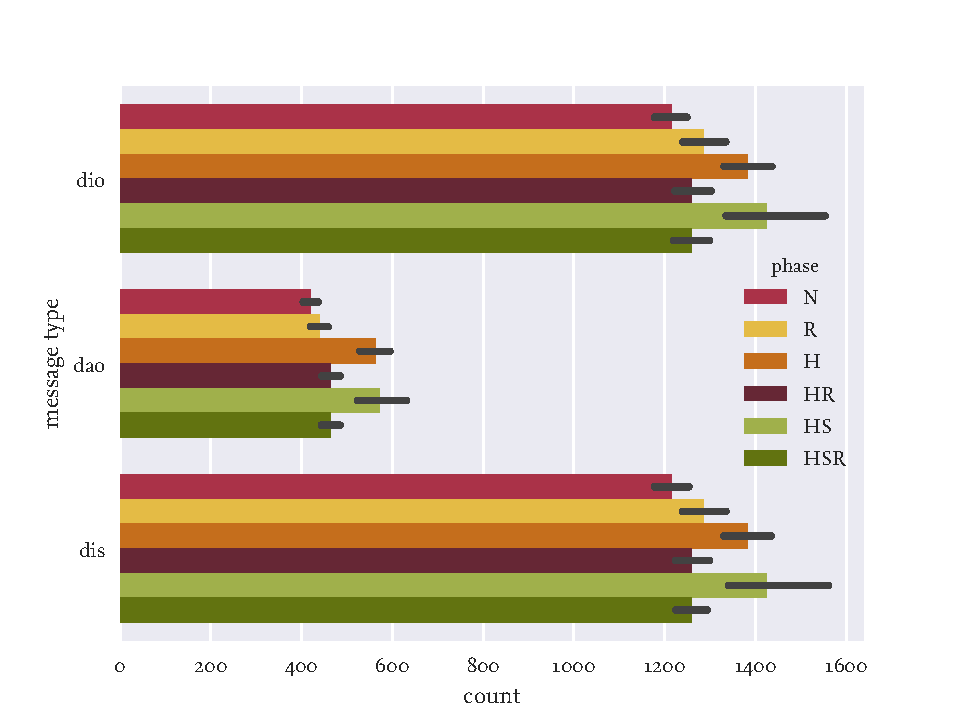
\includegraphics[height=0.3\textheight]{../images/performance-overhead.pdf}
  \caption{Overhead created by \ac{RPL} messages}
  \label{fig:overhead}
\end{figure}

For the phase R the overhead is higher than for the phase N, where no resets
occur. At the same time the inverse is true for the phases with hardened
implementations. Here the effect of an old state being restored and then
invalidated is later canceled out, when restoring the state after the node reset
occurred and actually less overhead is created than for the default implementation.

It should also be noted that there is no significant difference for the overhead
during the HR and HSR phases, which means that the implementation used in HS and
HSR does not offer a clear benefit over the implementation used in H and HR in
terms of message overhead.

\subsubsection{Consumption}

\begin{figure}
  \centering
  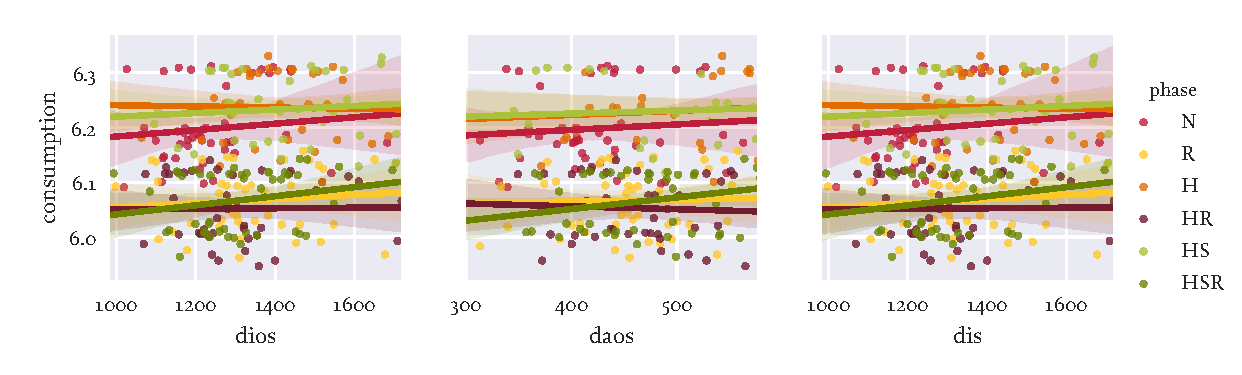
\includegraphics[width=\textwidth]{../images/performance-consumption.pdf}
  \caption{Relationship between overhead and energy consumption}
  \label{fig:overconsum}
\end{figure}

As can be seen from \autoref{fig:overconsum}, the number of control messages
correlate to the observed consumption. For a larger overhead, the total
consumption increases proportionally.
